%!TEX root = ../../prace.tex


\section{Elektrická síť}
\label{sec:energyNet}
Účel elektrické sítě ve hře vychází z~reálného světa. Chceme, aby bloky spolu mezi sebou uměly komunikovat skrze nějakou síť a~aby přes tuto síť bylo možné automaticky převádět energii, třeba z~bloku \RB{B6} do bloku \RB{B8}. Na elektrickou síť nebudeme klást žádné omezující požadavky (například limitací přenosové kapacity bloků tvořících danou síť).

Pokud budeme vycházet z~premisy, že každý blok je zapojen právě v~jedné elektrické síti a~všechny bloky v~rámci jedné elektrické sítě jsou mezi sebou vodivě spojeny (viz kapitola \ref{subsec:encomp}), tak nutně musíme dojít k~závěru, že při manipulaci s~bloky budeme muset elektrické sítě aktualizovat. Přidáním bloku bychom mohli vodivě propojit dvě či více sítí, při odebírání se nám daná elektrická síť může rozpadnout na více samostatných komponent. Těchto elektrických sítí může vznikat a~zanikat velké množství. Stačí si uvědomit, že k~bloku \RB{A1} o~maximální možné velikosti můžeme připojit až 600 bloků, které budou patřit do stejné sítě (pro každou stěnu máme 100 bloků stejného typu a~minimální velikosti, uspořádaných do šachovnicového vzoru). Pokud pak odebereme centrální blok, může nám vzniknout právě až 600 nových elektrických sítí. Navíc, díky počasí se může stát, že bloky budou odebírány ze světa zcela neuspořádaně (na základě náhodně udělovaného poškození). Musíme tedy vymyslet algoritmus, jak pro všechny bloky v~herním světě udržovat správné informace o~jejich síti.

Protože nemůžeme nic předpokládat o~tom, jak se budou bloky v~elektrické síti chovat, musíme při změně (přidání či odebrání) nějakého bloku v~síti provést přepočítání a~to i~u~sítě, která již může být přepočítávána. Nejjednodušší bude varianta na \textit{algoritmus vlny}. Jednotlivé sítě budeme podle potřeby odstraňovat či slévat. 

\pagebreak
Aby algoritmus vlny fungoval, je zapotřebí u~elektrické sítě a~každého bloku v~ní udržovat informaci o~stavu. Ty jsou tři:
\begin{itemize}
	\item Nevalidní
	\item Ve výpočtu
	\item Validní
\end{itemize}

Volba stavů je zřejmá a~vychází z~principů algoritmu vlny. Navíc tím můžeme požadovat, aby hra počítala s~tím, že elektrická síť a~bloky v~ní mohou být v~různých stavech a~tomu pak přizpůsobila svoji další funkcionalitu (například síť ve stavu \textit{ve výpočtu} nebude převádět zdroje sítě mezi bloky, které nejsou ve stavu \textit{validní} -- tedy těch, které již byly zpracovány algoritmem).

\subsection{Princip aktualizace sítě}

V předchozí části jsme zjistili, že nám může v~jednom okamžiku vzniknout velké množství sítí, jež je třeba aktualizovat. Navíc platí, že sítě mohou být rozsáhlé. Abychom co nejméně zasahovali do funkcionality aktualizovaných sítí, musíme nějakým způsobem zajistit, aby byla aktualizace sítí férová pro všechny sítě k~aktualizaci. Vzhledem k~tomu, že při nově vzniklém požadavku na aktualizaci sítě nevíme vůbec nic o~tom, které bloky nakonec v~dané síti budou, nemá smysl se zabývat myšlenkou upřednostňování aktualizace nějaké sítě vůči jiné, protože nemáme žádné faktické podklady pro to, jakou síť bychom měli upřednostnit.

Musíme tedy mít k~dispozici \textit{frontu sítí k~aktualizaci}. Každá síť z~této fronty si pak bude muset držet \textit{vlastní} frontu \textit{bloků k~aktualizaci}. V~algoritmu budeme postupně z~fronty vybírat sítě, provedeme u~nich krok algoritmu vlny a~případně je opět zařadíme do fronty. Tím zajistíme férovou aktualizaci pro všechny zúčastněné sítě.

Dále popíšeme, jak vypadá jeden krok algoritmu vlny. Jako sousedy budeme chápat bloky dostupné skrze vodivé spojení. Krok bude následující:

\begin{enumerate}
	\item Vyber blok \textbf{B} z~fronty bloků k~aktualizaci.
	\item Zkontroluj, že je \textbf{B} stále validní (zatímco \textbf{B} čekal ve frontě, mohl být mezitím zničen bouří kyselého deště). Pokud není validní, skonči.
	\item \textbf{B} označ jako \textit{Validní}.
	\item Pro všechny sousedy \textbf{S} bloku \textbf{B} se podívej na jejich síť a~stav bloku a~vykonej akci dle tabulky \ref{table:networkAlg}.
\end{enumerate}


\begin{table}[h]
\centering
\begin{tabular}{| l | l | l | l |}
	\hline
	Síť  \textbf{S}~~~$\backslash$~~ Stav \textbf{S}	& Nevalidní			& Ve výpočtu	& Validní 			\\ \hline
	Stejná jako \textbf{B}					& Naplánuj 	 		& Nic 			& Nic 	     			\\ \hline
	Jiná než \textbf{B} 						& \uv{Ukradni} a~naplánuj & Nic 			& Spoj sítě do jedné   	\\ \hline
\end{tabular}
\caption{Požadované bloky a~jejich základní vlastnosti}
\label{table:networkAlg}
\end{table}

\FloatBarrier

Abychom dobře pochopili význam akcí v~tabulce \ref{table:networkAlg}, měli bychom jednotlivé akce podrobněji popsat. Začněme situací, kdy je \textbf{S} ve stejné síti jako \textbf{B}.

Pokud je stav \textbf{S} \textit{Nevalidní}, pak musíme tento nalezený blok přidat do fronty bloků k~aktualizaci. Pokud je ve stavu \textit{Ve výpočtu}, pak je již naplánován, ale ještě nebyl zpracován (jinak by byl označen jako \textit{Validní}). Pokud je označen jako \textit{Validní}, byl již zpracován. Tyto kroky odpovídají standardnímu výpočtu algoritmu vlny. Pojďme se nyní podívat na situace, kdy jsou sítě \textbf{S} a~\textbf{B} \textit{odlišné}.

Pokud je stav \textbf{S} \textit{Nevalidní}, pak můžeme tento blok přiřadit do sítě \textbf{B} a~naplánovat ho ke zpracování. Určitě platí, že blok není v~žádné frontě ke zpracování (jinak by měl jiný stav). Pokud bychom ho \uv{neukradli}, zbytečně bychom tím ztratili cyklus kroku algoritmu. Navíc, jak je zmíněno v~části \ref{subsec:reac}, při odebírání je původní síť ponechána netknutá a~bloky jsou zneplatněny. Bez této vlastnosti bychom neuměli \uv{rozebrat} původní síť. Pokud je \textbf{S} ve stavu \textit{Ve výpočtu}, pak je již naplánován a~nemusíme dělat nic. Zde je důležitý fakt, že \textbf{S} bude někdy v~budoucnu vykonávat 4. krok algoritmu vlny a~tudíž nutně narazí na \textbf{B}, jakožto svého souseda s~jinou sítí. Ale protože \textbf{B} bude v~té době ve stavu \textit{Validní}, případ se tím převede na zbývající možnost. Když je \textbf{S} označen jako \textit{Validní}, pak musíme obě sítě spojit do jedné, protože všechny \textit{Validní} bloky z~obou sítí jsou propojeny skrze vodivé spojení \textbf{B} a~\textbf{S} a~tudíž musí mít i~stejnou síť.



\subsection{Reakce na přidání a~odebrání bloku}
\label{subsec:reac}
\subsubsection{Přidávání bloku}
Přidání bloku do systému elektrických sítí je jednoduché. Platí, že každý blok přidaný do herního světa si při přidávání vytvoří svoji vlastní elektrickou síť. Ta je pak přidána mezi všechny elektrické sítě v~herním světě a~je naplánovaná její \textit{aktualizace}. 

\subsubsection{Odebírání bloku}
Každý odebíraný blok z~herního světa vždy zneplatní celou síť, ke které je připojen (takže všechny bloky jsou v~nevalidním stavu), a~pro všechny jeho sousedy vytvoří nové sítě, které následně naplánuje k~\textit{aktualizaci}. Po dokončení všech aktualizačních výpočtů všech elektrických sítí je pak původní elektrická síť odstraněna. Dříve tak nesmíme učinit, protože bychom přišli o~vazby na bloky. Zde je také vidět, proč musíme umět \uv{krást} bloky.

\subsection{Optimalizace algoritmu}

Jak je vidět z~předchozí kapitoly, výpočtů v~aktualizaci může být velmi mnoho. Nesmíme však dopustit, aby se nám při přepočítávání začala hra zpomalovat či přímo zasekávat\footnote{Tato situace může snadno nastat, protože herní a~renderovací smyčky se na konci svých cyklů synchronizují, aby pro výpočet dalšího framu začínaly stejně.}. Opět máme více možností řešení, jak se k~tomuto problému postavit. 

Jedním z~možných řešení je spuštění výpočtů na samostatném výpočetním vlákně. Zde bohužel narážíme na problém, že výpočty ve vláknech v~\UEu{} nemohou přímo přistupovat k~herním objektům a~tudíž je nutné používat pomocných datových struktur a~výsledky poté zpětně propagovat. Kromě toho také narážíme na problém, kdy v~případě velmi silné bouře kyselých dešťů bude nejspíše často nutné výpočet předčasně ukončit a~spustit znovu.

Algoritmus bude mít přidělené nějaké maximální kvantum času, řekněme tolik, aby při jeho výpočtech hra dosahovala alespoň 30 snímků za sekundu. Pokud toto kvantum vyčerpá, nebude začínat další výpočty a~naplánovanou práci nechá do dalšího cyklu herní smyčky. Tím vcelku jednoduchým a~elegantním způsobem zajistíme aktualizace i~pro velice rozsáhlé sítě bez negativního vlivu na plynulost hry.








\section{Bloky v~herním světě}
\label{sec:blocksWorld}

Způsobů, jak reprezentovat bloky ve světě, je více, takže bychom měli jednotlivé varianty porovnat a~vyhodnotit. V~této chvíli si také musíme určit, jak velký chceme náš herní svět mít. Na základě tohoto důležitého požadavku budeme posuzovat vhodnost jednotlivých implementací. My jsme se rozhodli, že hráči nabídneme rozsáhlý svět čtvercového půdorysu o~rozloze $100\,\ km^2$ a~výšky $5\,\ km$. V~takto rozsáhlém herním světě bude mít hráč dostatek prostoru pro stavbu svých budov, a~to i~v~případě, že se v~budoucnu rozhodneme rozšiřovat hru o~nové bloky a~herní vlastnosti. Zároveň s~tím si ale uvědomujeme, že správně by hra měla řešit takto velký svět tak, aby i~velké množství bloků hru nezpomalovalo či dokonce neshodilo celou hru (třeba z~nedostatku paměti RAM). Nicméně jak jsme zmínili v~kapitole \ref{subsec:bloky}, budeme v~této práci očekávat takové množství bloků, jejichž počet hra bez problémů zvládne.

Námi definované hranice herního světa se u~bloků projeví tak, že v~rámci herního světa můžeme mít až $50~000 * 50~000 * 25~000$ bloků jednotkové velikosti, což je opravdu mnoho. Nejprve se tedy zaměříme na to, jak vůbec můžeme bloky reprezentovat a~zároveň s~tím budeme řešit, jak se vypořádat s~různými rozměry bloků.

\subsection{Použití dvourozměrného pole}

Představme si, že bychom herní svět reprezentovali polem. Pak bychom potřebovali 62~500~\textit{miliard} ukazatelů, z~nichž by naprostá většina byla prázdných (\textit{NULL}ových). Pro jednoduchost počítejme, že jeden ukazatel má velikost 4B a~že 1 kB je roven 1000 B. Pak dostáváme, že bychom potřebovali alokovat 250~TB dat. To vidíme jako problém, takže se zkusme zaměřit na efektivnější datové struktury.

\subsection{Stromové struktury}
\label{subsec:trees}

Jako rozumný nápad se jeví použití stromových struktur, které nám budou reprezentovat svět podle skutečně zabraných pozic v~herním světě. Kdybychom povolili volnou počáteční rotaci, zřejmě bychom museli přistoupit k~nějaké variantě \textit{clusterů}, tedy shluků bloků ve stejné ortogonální mřížce. Protože tuto vlastnost nepovolujeme, můžeme se zabývat jinými datovými strukturami. Běžně používané datové struktury ve hrách jsou například:
\pagebreak
\begin{itemize}
	\item Octree
	\item K-D stromy
\end{itemize}

Pojďme si tedy tyto možnosti rozebrat a~zhodnotit v~kontextu naší hry.

\subsubsection{Octree}
Octree je stromová datová struktura, ve které vrchol reprezentuje nějaký objem a~jeho 8 potomků tento objem rovnoměrně dělí na menší části. Obvykle vrcholy této struktury reprezentují krychle v~nějakém prostoru. Pokud se zamyslíme, jak by náš svět byl v~této struktuře reprezentován, dojdeme k~tomu, že kořenový vrchol této struktury by měl 4 potomky vždy prázdné. Ačkoliv to není nijak zásadní nevýhoda, podívejme se na alternativní řešení.

\subsubsection{K-D strom}
K-D strom je datová struktura, která je velmi podobná Octree, ale na rozdíl od ní má pouze 2 potomky. Vrchol, který se nachází v~nějaké hladině, totiž svůj objem rozdělí do dvou polovin v~závislosti na dané hladině. Takto je možné reprezentovat vícedimenziální prostory, kdy jednotlivé hladiny reprezentují dělení pro jednotlivé souřadnice. Každá následující hladina této struktury pak představuje dělení podle následující souřadnice v~daném prostoru. Pro n-dimenzionální prostor pak (n+1) hladina (počítáno od jedné) opět dělí prostor podle první souřadnice.

\subsubsection{Vlastní rozšíření K-D stromu}
K-D strom je pro naši situaci vhodnější, protože při správné implementaci této struktury můžeme změnit rozměry herního světa (pokud to bude potřeba) a~nebudeme muset měnit implementaci reprezentace bloků v~herním světě. V~rámci našeho rozšíření navrhujeme, aby si jednotlivé vrcholy uchovávaly informaci o~reprezentované části herního světa v~podobě Min-Max boxu\footnote{Jako Min-Max box budeme chápat strukturu, která je popsána dvěma vektory, které představují minimální a~maximální hranice. Ve 2D prostředí by to byl obdélník s~udáním levého dolního rohu a~pravého horního rohu.}. Tuto vlastnost pak využijeme pro rychlé dotazování nad tímto stromem (například při kontrole, zda je možné nějaký blok umístit na nějakou pozici v~herním světě). Navíc budeme chtít, aby byla hloubka stromu co nejmenší, takže navrhujeme optimalizaci, kdy blok ve stromě může být v~daném vrcholu uložen jako \uv{jedináček}. Tento blok může být umístěn kdekoliv v~prostoru, který daný vrchol reprezentuje. 

\subsection{Reprezentace bloku}

Abychom si usnadnili indexování bloků, budeme uvažovat, že bloky jsou\linebreak v~osách X a~Y indexovány v~intervalu <-25~000, 25~000>. V~ose Z~(tedy vertikální ose) budeme bloky indexovat v~intervalu <0, 25~000> a~indexy ve všech osách budou celočíselné. Dále určíme fakt, že jednotkový blok na herních souřadnicích [0, 0, 0] bude v~\UEu{} reprezentován na pozici [0, 0, 0]. 

\subsubsection{Střed bloku a~škálování}
Pro potřeby porozumění následujícího textu se přesuneme z~3D prostoru, ve kterém v~\UEu{} pracujeme, do 1D prostoru. Jednotkovou úsečkou budeme rozumět úsečku o~délce $20\,\ cm$. Tuto jednotkovou úsečku umístíme na osu tak, že střed úsečky je přesně ve středu osy. Tudíž kraje jednotkové úsečky jsou v~bodech [-10], [10].

Nyní potřebujeme určit body osy, ke kterým budeme střed jednotkové úsečky přichytávat. To budou přesně $k$-násobky délky jednotkové úsečky pro libovolné celočíselné $k$. Nyní můžeme říci, že pokud budeme chtít umístit jednotkovou úsečku na $n$-tý index osy, střed této jednotkové úsečky bude v~bodě $n * 20$ a~kraje jednotkové úsečky budou v~bodech $[(n * 20) -- 10]$ a~$[(n * 20) + 10]$. Vidíme, že kraje jednotkové úsečky jsou správně zarovnané a~pro $n = 0$ odpovídají umístění jednotkové úsečky.

Nyní si představme situaci, že chceme na osu umístit jednotkovou úsečku zvětšenou na \textit{dvojnásobek} (označme ji \textbf{D}). Zvětšování je symetrické dle středu a~po umístění \textbf{D} na \textit{nultý} index osy dostáváme, že kraje \textbf{D} jsou v~bodech [-20], [20]. Nyní vidíme, že kraje \textbf{D} nejsou správně zarovnané, protože prochází námi definovanými body pro přichytávání. Kdybychom teď chtěli na index 1 umístit jednotkovou úsečku, obě úsečky se nám protínají a~to je špatně -- chceme dosáhnout toho, aby i~po libovolném zvětšení jednotkové úsečky byla tato úsečka správně zarovnaná.

Je důležité si uvědomit, že problém z~předchozího odstavce vzniká (díky symetrii zvětšování) pouze při škálování \textit{sudým} číslem. Pro tato čísla musíme udělat to, že střed bloku si \uv{virtuálně} posuneme tak, abychom celou škálovanou úsečku správně zarovnali do námi definovaných hranic (tento virtuální střed budeme správně přichytávat k~ose). Při určování virtuálního středu se budeme řídit pravidlem \uv{nejbližšího nižšího} možného středu. 

Demonstrujme posouvání virtuálního středu následujícím příkladem.\linebreak Vezměme si čtyřnásobně zvětšenou jednotkovou úsečku, označme si ji jako \textbf{Č}. Budeme ji chtít umístit na \textit{nultý} index osy. Bez posouvání středu bychom řekli, že hranice úsečky jsou v~bodech [-40], [40]. Představme si \textbf{Č} rozloženou na jednotkové úsečky, zleva indexované od 0. Nyní máme střed na indexu [$1,5$], tedy \textit{mezi} jednotkovými úsečkami 1 a~2. Pravidlem \uv{nejbližšího nižšího} virtuálně posuneme střed \textbf{Č} na index [1]. Když pak jednotkou úsečku na indexu [1] správně přichytíme k~ose, hranice se nám posunou o~$10\,\ cm$ doprava, kraje \textbf{Č} budou v~bodech [-30], [50] a~tím dosáhneme správného zarovnání.

Posledním krokem je rozšíření výše uvedených myšlenek všechny tři souřadnice 3D prostoru. Nyní už víme, jaký způsobem budeme řešit zarovnání bloku o~nějaké škále na daných \textit{herních} souřadnicích. Zároveň z~toho můžeme vidět, jakým způsobem budeme postupovat při převodu z~našeho souřadnicového systému do systému souřadnic v~rámci \UEu{}.
 
\subsubsection{Důsledky škálování}

Z výše uvedených faktů je vidět, že ve hře budou muset existovat pravidla pro výpočty mezi souřadnicovým systémem naší hry a~souřadnicovým systémem \UEu{}. Dále z~toho vyplývá, že pokud má blok netriviální škálování, dle výše uvedených pravidel může inherentně \uv{zabrat} některé pozice v~našem souřadnicovém systému a~jiné bloky pak tento prostor nemohou obývat. To je skvělý výsledek, protože tím máme vyřešené konkrétní pozice a~nemohou nám nastat konflikty umístění bloků.

Dalším důležitým důsledkem je způsob rotací škálovaných bloků. Budeme chtít, aby blok rotoval vzhledem k \textit{virtuálnímu} středu. 

Dále máme usnadněné výpočty hranic bloku vůči globální souřadnicovému systému \UEu{}. K tomu nám stačí umístění v~našem souřadnicovém systému, velikosti a~rotaci bloku. Výsledkem pak může být Min-Max box, který můžeme použít pro dotazy nad naším K-D stromem. Jednoduchým a~rychlým výpočtem pak můžeme analyzovat, jestli mají nějaké dva bloky nějaký netriviální průnik, jestli se dotýkají apod.


\subsubsection{Důsledky reprezentace bloků na herní svět}

Budeme chtít, aby jednotlivé vrcholy našeho K-D stromu znaly svoji reprezentaci v~podobě Min-Max boxu. Tím získáme výhodu rychlého vyhodnocení dotazů (kupříkladu zda je možné umístit nový blok na nějaké souřadnice udané hráčem). Dále, budeme chtít, aby bloky měly vazbu na náš K-D strom. Cílem je dosáhnout toho, aby blok mohl vyhledávat své sousedy \uv{odspodu} a~jejich hledání tak bylo velmi rychlé.


\subsection{Zapojení do rozpoznávání tvarů}

Vzhledem k~dynamicky škálovatelným blokům budeme požadovat, aby bylo možné bloky skládat do tvarů libovolným splňujícím způsobem. Dobře je to vidět na následujícím obrázku \ref{fig:konfig}:

\begin{figure}[!ht]\centering
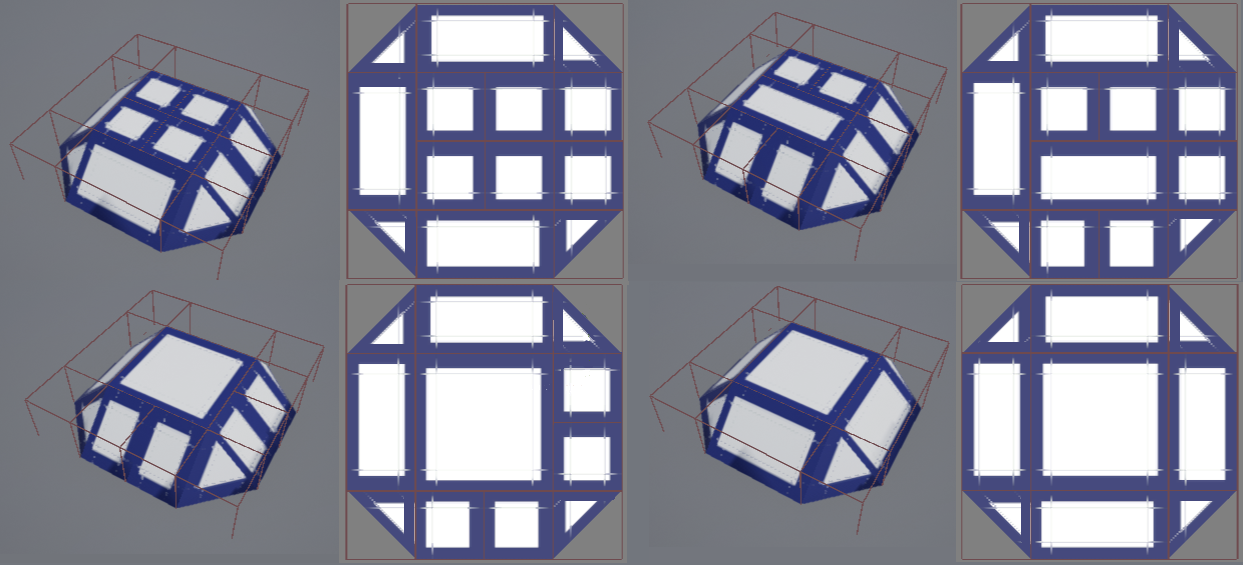
\includegraphics[ width=140mm]{../img/analysis/konfigurace}

\caption{Ekvivalentní konfigurace tvaru. Zdroj: StackOverflow.com~\citep{so_pattern}}
\label{fig:konfig}

\end{figure}

\FloatBarrier

Všechny tvary z~obrázku \ref{fig:konfig} by měly dohromady tvořit stejný tvar, ačkoliv splnění tohoto tvaru bylo u~každého tvaru rozdílné. Tento přístup však přináší mnoho problémů. Pro příklad uvažme rozklad bloku \RB{A5} netriviální velikosti (kupříkladu [2,~1,~2], tedy šířky jednotkového bloku). Je zřejmé, že stejného tvaru je možné dosáhnout použitím dvou stejných bloků velikosti [1,~1,~1] a~jednoho bloku \RB{A2} velikosti [1,~1,~1] (pokud budeme uvažovat, že tyto dva bloky je možné vzájemně kombinovat).

Z předchozích poznatků vyplývá, že definice nějakého komplexního tvaru, složeného z~různých typů bloků
(TODO dokončit)


